\documentclass[letterpaper,sansserif,tightsqueeze]{rpg-module}

\usepackage{parskip}                                                            % Add spacing between paras instead of indents
\usepackage[font=bf]{caption}

\title{Excavated Thaumaturgy}

% Compress title spacing compared to default

\addtolength{\topmargin}{-0.3cm}
\addtolength{\textheight}{0.7cm}

\begin{document}

\twocolumn

\title{Excavated Thaumaturgy}

\subtitle{Optional Rules and Miscellaneous Artifacts}

\coverimage{weapons.png}

\abstract{$\ll$Abstract in construction$\gg$.}


\maketitle

\vspace{0.5cm}
\part*{Optional Rules for Combat}
\vspace{0.5cm}

\begin{center}
	
\includegraphics[width = 0.3\linewidth]{dead.png}
\end{center}
\section{Bleeding out}
\textit{This rule is intended to add an unpredictable element to dying in battle.}

Instead of dying immediately when a damaging effect causes your HP to go to 0 or lower, you start bleeding out:
\begin{itemize}
	\item You immediately gain a pool of \textit{bleed out points}, this pool starts at 0.
	\item You have to stay prone and cannot act except for moving 5 feet.
	\item The GM rolls a d6 whenever you would normally act and increases your bleed out points by the rolled result without disclosing the either the roll or the total.
	\item The GM rolls another d6 and adds the result to the PC's total any time the PC is hit by a damaging effect.
	\item When the total is equal to or exceeds the PC's Constution score, the PC has bled out and dies.
\end{itemize}
\textbf{Applying pressure:} Other players can stop the bleeding by spending their turn taking care of the bleeding PC, the PC then becomes \textit{Stabilized}, this state is negated when the PC takes damage.

\textbf{Healing:} A downed PC can only be healed - magically or non-magically - when he or she has been stabilized. The bleed out pool is reset once the PC is healed, the bleed out score does not affect the amount of HP restored.

\newpage

\vspace{0.5cm}
\part*{Cursed Artifacts}
\vspace{0.5cm}

\begin{center}
	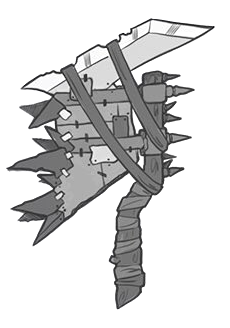
\includegraphics[width = 0.5\linewidth]{Garthruks_axe.png}
\end{center}
\section{The Axe of Garthruk}
\textit{A blackened axe made with crude green metal. It angrily shakes when approached.}

Garthruk the Orc Chief is captured within the axe. He wants to challenge the great and mighty, and escape his metal prison.

Abilities:
\begin{itemize}
	\item \textbf{Orcish Strength:} The wielder's muscles bulge and he suddenly can perform orcish feats of strength.
	\item \textbf{Possession:} When triggered, Garthruk will try to possess the wielder. Save against Paralysis or be possessed for 3d6 minutes by a raging Orc. Possession occurs when one of the following conditions is met:
	\begin{itemize}
		\item Attempting to get rid of the axe (automatic possession, no save allowed).
		\item Evading a mighty foe.
		\item Failing to protect your honor.
	\end{itemize}
	\item \textbf{Corruption:} Every failed save gives the wielder an Orc point. After the wielder reached his Orc threshold - 2d6 rolled in secret by the GM after touching the axe - the wielder will count as being an Orc instead of his/her former race.
\end{itemize}
Stages: 
\begin{itemize}
	\item \textbf{Stage 1 (1 Orc point}:) The wielder's face becomes cruder ever so slightly. His/her speech becomes rougher. 
	\item \textbf{Stage 2 (Orc threshold/2, rounded down):} The wielder becomes a half-Orc.
	\item \textbf{Stage 3: (Orc threshold):} The wielder is now a full-fledged Orc.
\end{itemize}

\end{document}
